\documentclass[11pt,t]{beamer}
\usetheme{default}
\beamertemplatenavigationsymbolsempty
\hypersetup{pdfpagemode=UseNone} % don't show bookmarks on initial view
\usefonttheme{professionalfonts}
\usefonttheme{serif}
\usepackage{fontspec}
\setmainfont{Ubuntu}
\setmonofont{Ubuntu Mono}
\usepackage{url}
\usepackage[english]{babel}
\usepackage{verbatim}
%\usepackage{times}
\usepackage{graphicx}
\usepackage[utf8]{inputenc}
%\usepackage[T1]{fontenc}
\usepackage{listings}
\usepackage{mathtools}
\usepackage{color}
\usepackage{minted}
\usemintedstyle{vim}
\usepackage{tikz}
\usepackage[underline=false]{pgf-umlsd}
\usetikzlibrary{positioning, fit, calc, shapes, arrows, shadows}
\usepgflibrary{arrows}
\definecolor{lightgray}{gray}{0.70}

\definecolor{fore}{RGB}{249,242,215}
\definecolor{back}{RGB}{51,51,51}
\definecolor{title}{RGB}{200,0,90}
\setbeamercolor{titlelike}{fg=title}
\setbeamercolor{normal text}{fg=fore,bg=back}

\definecolor{foreground}{RGB}{255,255,255}
\definecolor{background}{RGB}{24,24,24}
\definecolor{title}{RGB}{107,174,214}
\definecolor{gray}{RGB}{155,155,155}
\definecolor{subtitle}{RGB}{102,255,204}
\definecolor{hilight}{RGB}{102,255,204}
\definecolor{vhilight}{RGB}{255,111,207}
\setbeamercolor{titlelike}{fg=title}
\setbeamercolor{subtitle}{fg=subtitle}
\setbeamercolor{institute}{fg=gray}
\setbeamercolor{normal text}{fg=foreground,bg=background}
\setbeamercolor{item}{fg=foreground} % color of bullets
\setbeamercolor{subitem}{fg=lightgray}
\setbeamercolor{itemize/enumerate subbody}{fg=lightgray}
\setbeamertemplate{itemize subitem}{{\textendash}}
\setbeamerfont{itemize/enumerate subbody}{size=\footnotesize}
\setbeamerfont{itemize/enumerate subitem}{size=\footnotesize}
\newcommand{\funcname}[1]{
	{\color{yellow!30} #1}
}
\newcommand{\cipher}[1]{
	{\color{blue!30} #1}
}
\renewcommand*{\thefootnote}{\fnsymbol{footnote}}
\setbeamertemplate{footline}[text line]{%
  \parbox{\linewidth}{\vspace*{-8pt}
  \hfill
  %\insertshortauthor
  \hfill
  \insertframenumber\ of \inserttotalframenumber}}
\setbeamertemplate{navigation symbols}{}

\title{Cryptography and secure\footnotemark[1] systems \\\vspace{0.5cm} \footnotemark[1] 
{\small in the real world}}
\author{Vsevolod Stakhov \\ \url{vsevolod@FreeBSD.org}}

\newcommand{\bloodymess}[7][0]{
  \stepcounter{seqlevel}
  \path
  (#2)+(0,-\theseqlevel*\unitfactor-0.7*\unitfactor) node (mess from) {};
  \addtocounter{seqlevel}{#1}
  \path
  (#4)+(0,-\theseqlevel*\unitfactor-0.7*\unitfactor) node (mess to) {};
  \draw[->,>=angle 60] (mess from) -- (mess to) node[midway, above]
  {#3};

  \if R#5
    \node (#3 from) at (mess from) {\llap{#6~}};
    \node (#3 to) at (mess to) {\rlap{~#7}};
  \else\if L#5
         \node (#3 from) at (mess from) {\rlap{~#6}};
         \node (#3 to) at (mess to) {\llap{#7~}};
       \else
         \node (#3 from) at (mess from) {#6};
         \node (#3 to) at (mess to) {#7};
       \fi
  \fi
}
\begin{document}

\begin{frame}[plain]
  \titlepage
\end{frame}

\begin{frame}
\frametitle{How expensive is encryption nowadays}
\begin{itemize}
  \item<1-> New hardware:
  \begin{itemize}
    \item specialized encryption instructions (AES-NI)
    \item vectorized operations (SSE, AVX, AVX2, AVX512)
  \end{itemize}
  \item<2-> New algorithms:
  \begin{itemize}
    \item optimized chaining mode (e.g. CTR instead of CBC)
    \item optimized algorithms (from \cipher{3DES} to \cipher{ChaCha20})
  \end{itemize}
  \item<3-> New protocols
\end{itemize}
\end{frame}

\begin{frame}
\frametitle{How expensive is encryption nowadays}
\framesubtitle{Hardware performance}
2011: Westmere (SSE4, AES-NI):
\begin{figure}[H]
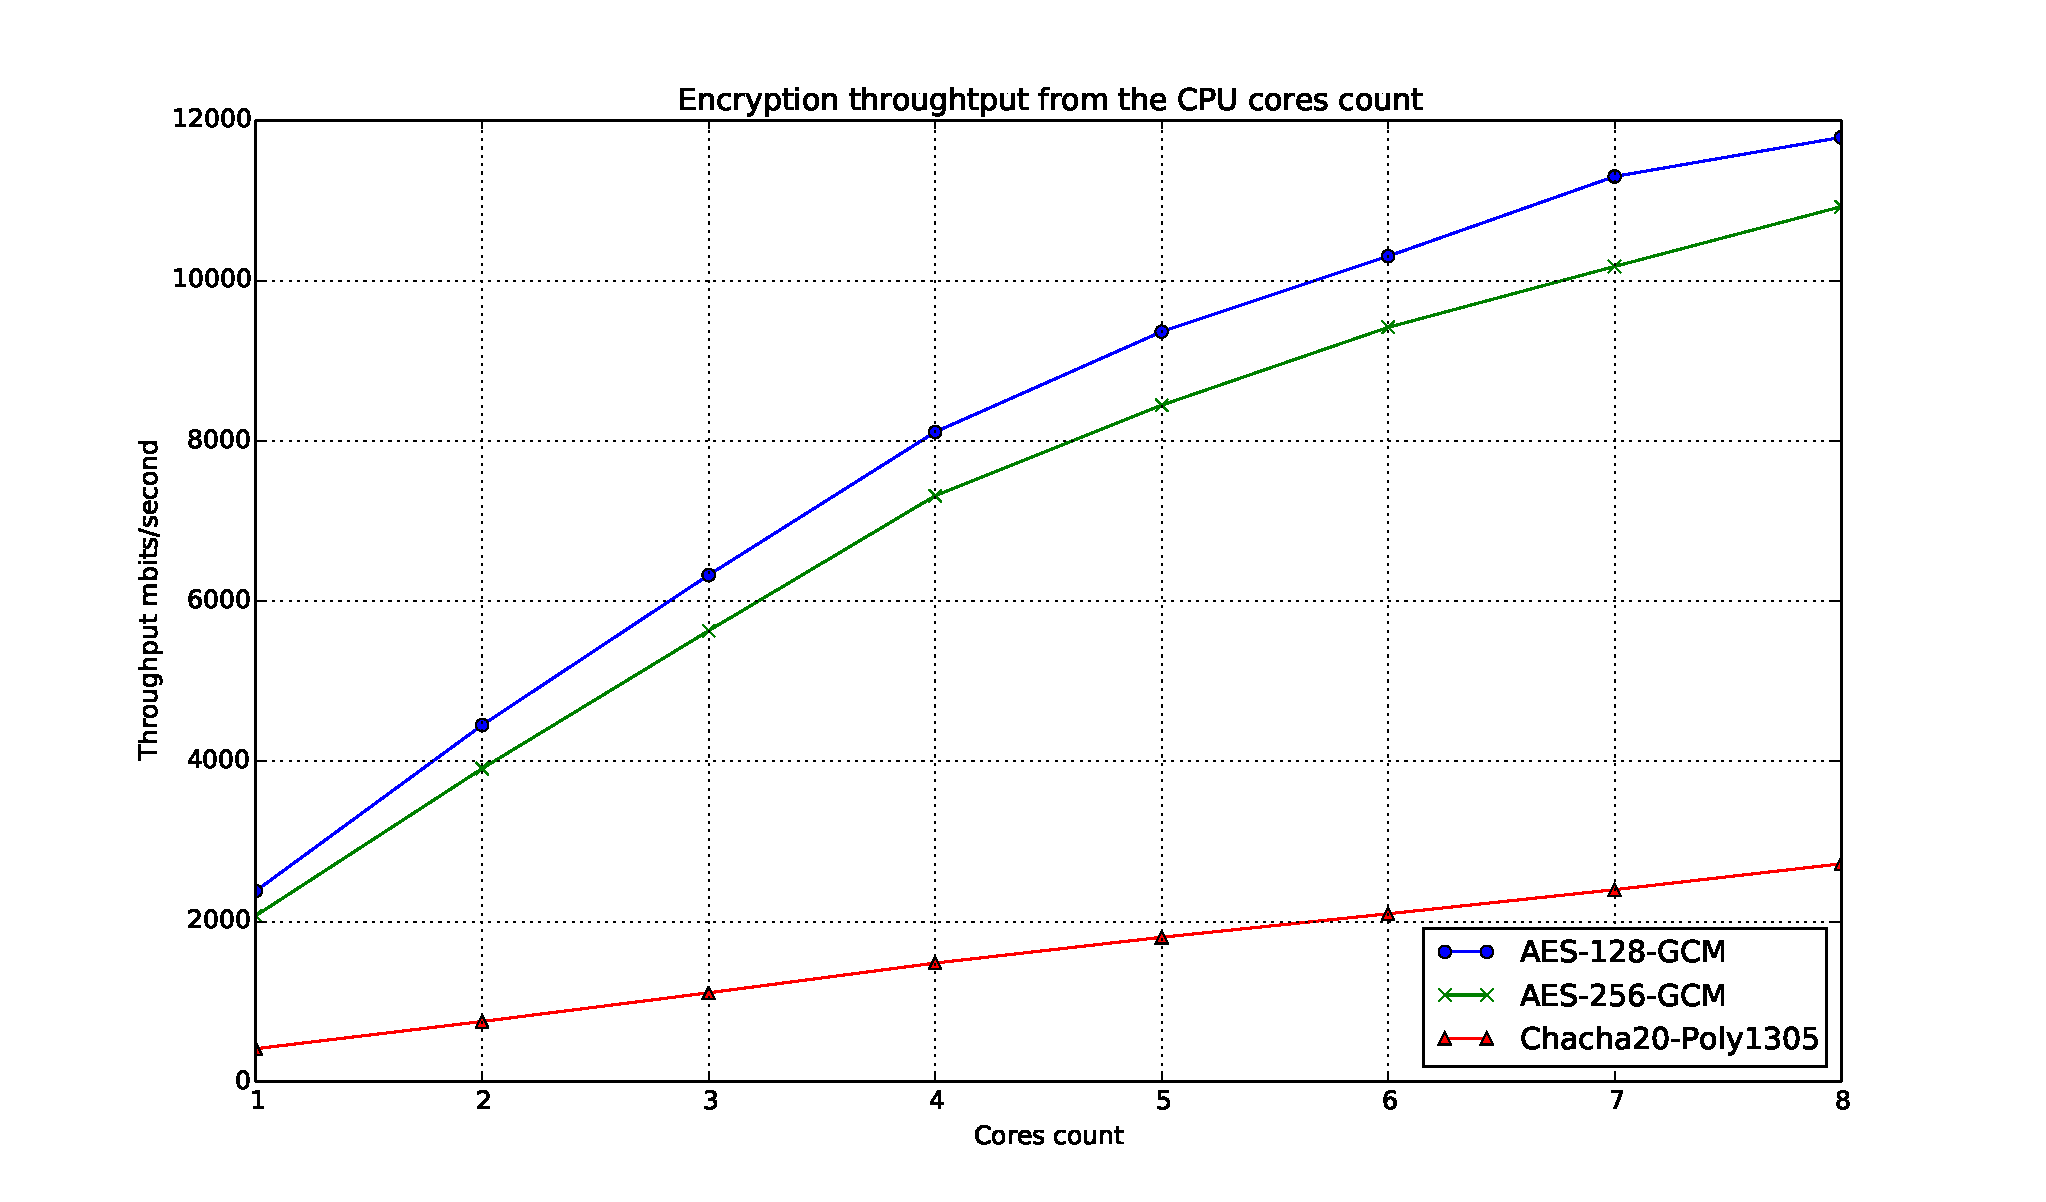
\includegraphics[height=0.6\textheight]{perf-e7.pdf}
\caption{XeonE7, 2.1 GHz, 8 CPU cores}
\end{figure}
\end{frame}

\begin{frame}
\frametitle{How expensive is encryption nowadays}
\framesubtitle{Hardware performance}
2012: Sandy Bridge (AVX, AES-NI):
\begin{figure}[H]
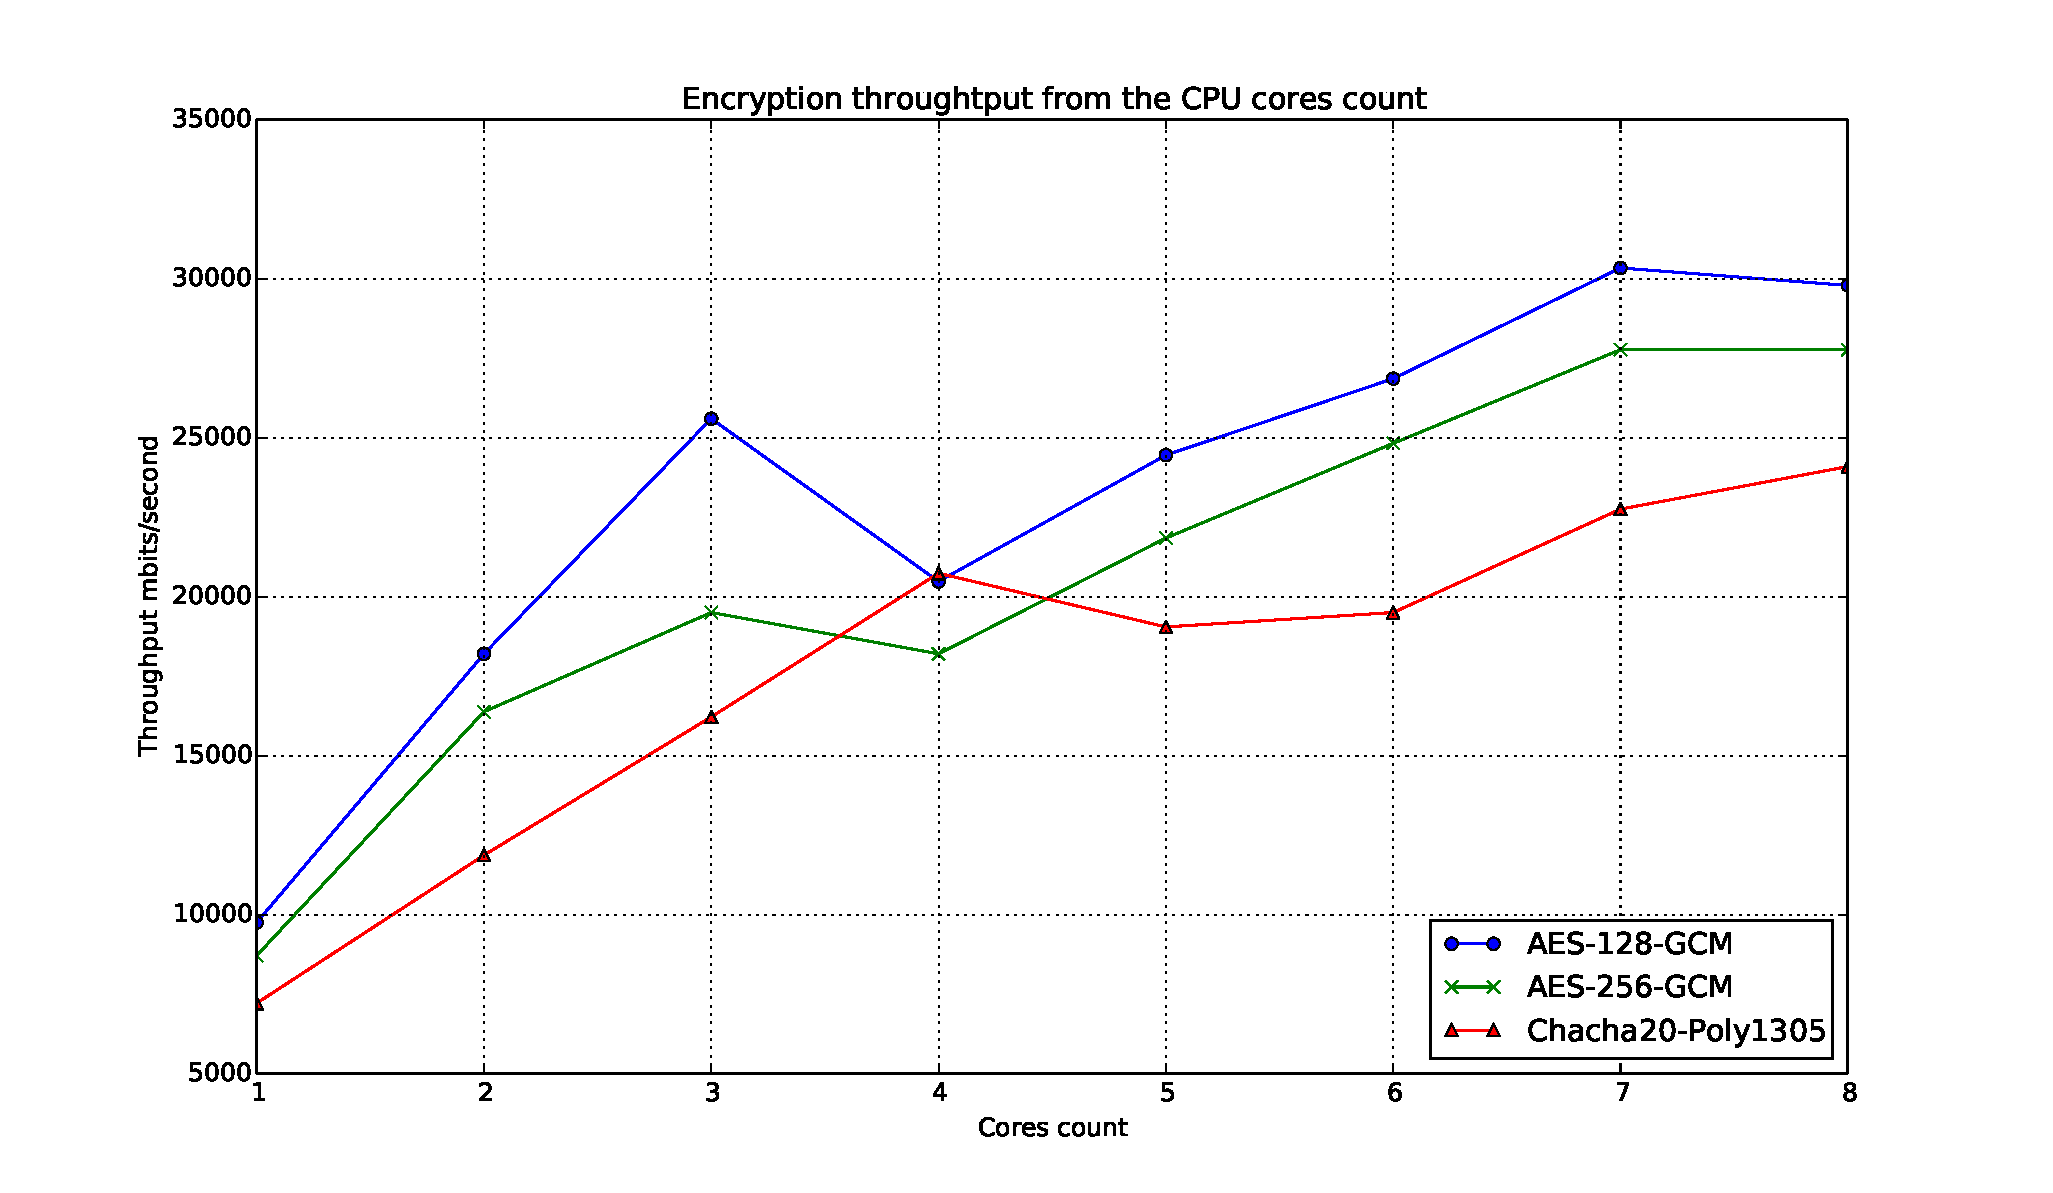
\includegraphics[height=0.6\textheight]{perf-e3.pdf}
\caption{Xeon E3, 3.4 GHz, 8 CPU cores}
\end{figure}
\end{frame}

\begin{frame}
\frametitle{How expensive is encryption nowadays}
\framesubtitle{Hardware performance}
2013: Haswell (AVX2, AES-NI):
\begin{figure}[H]
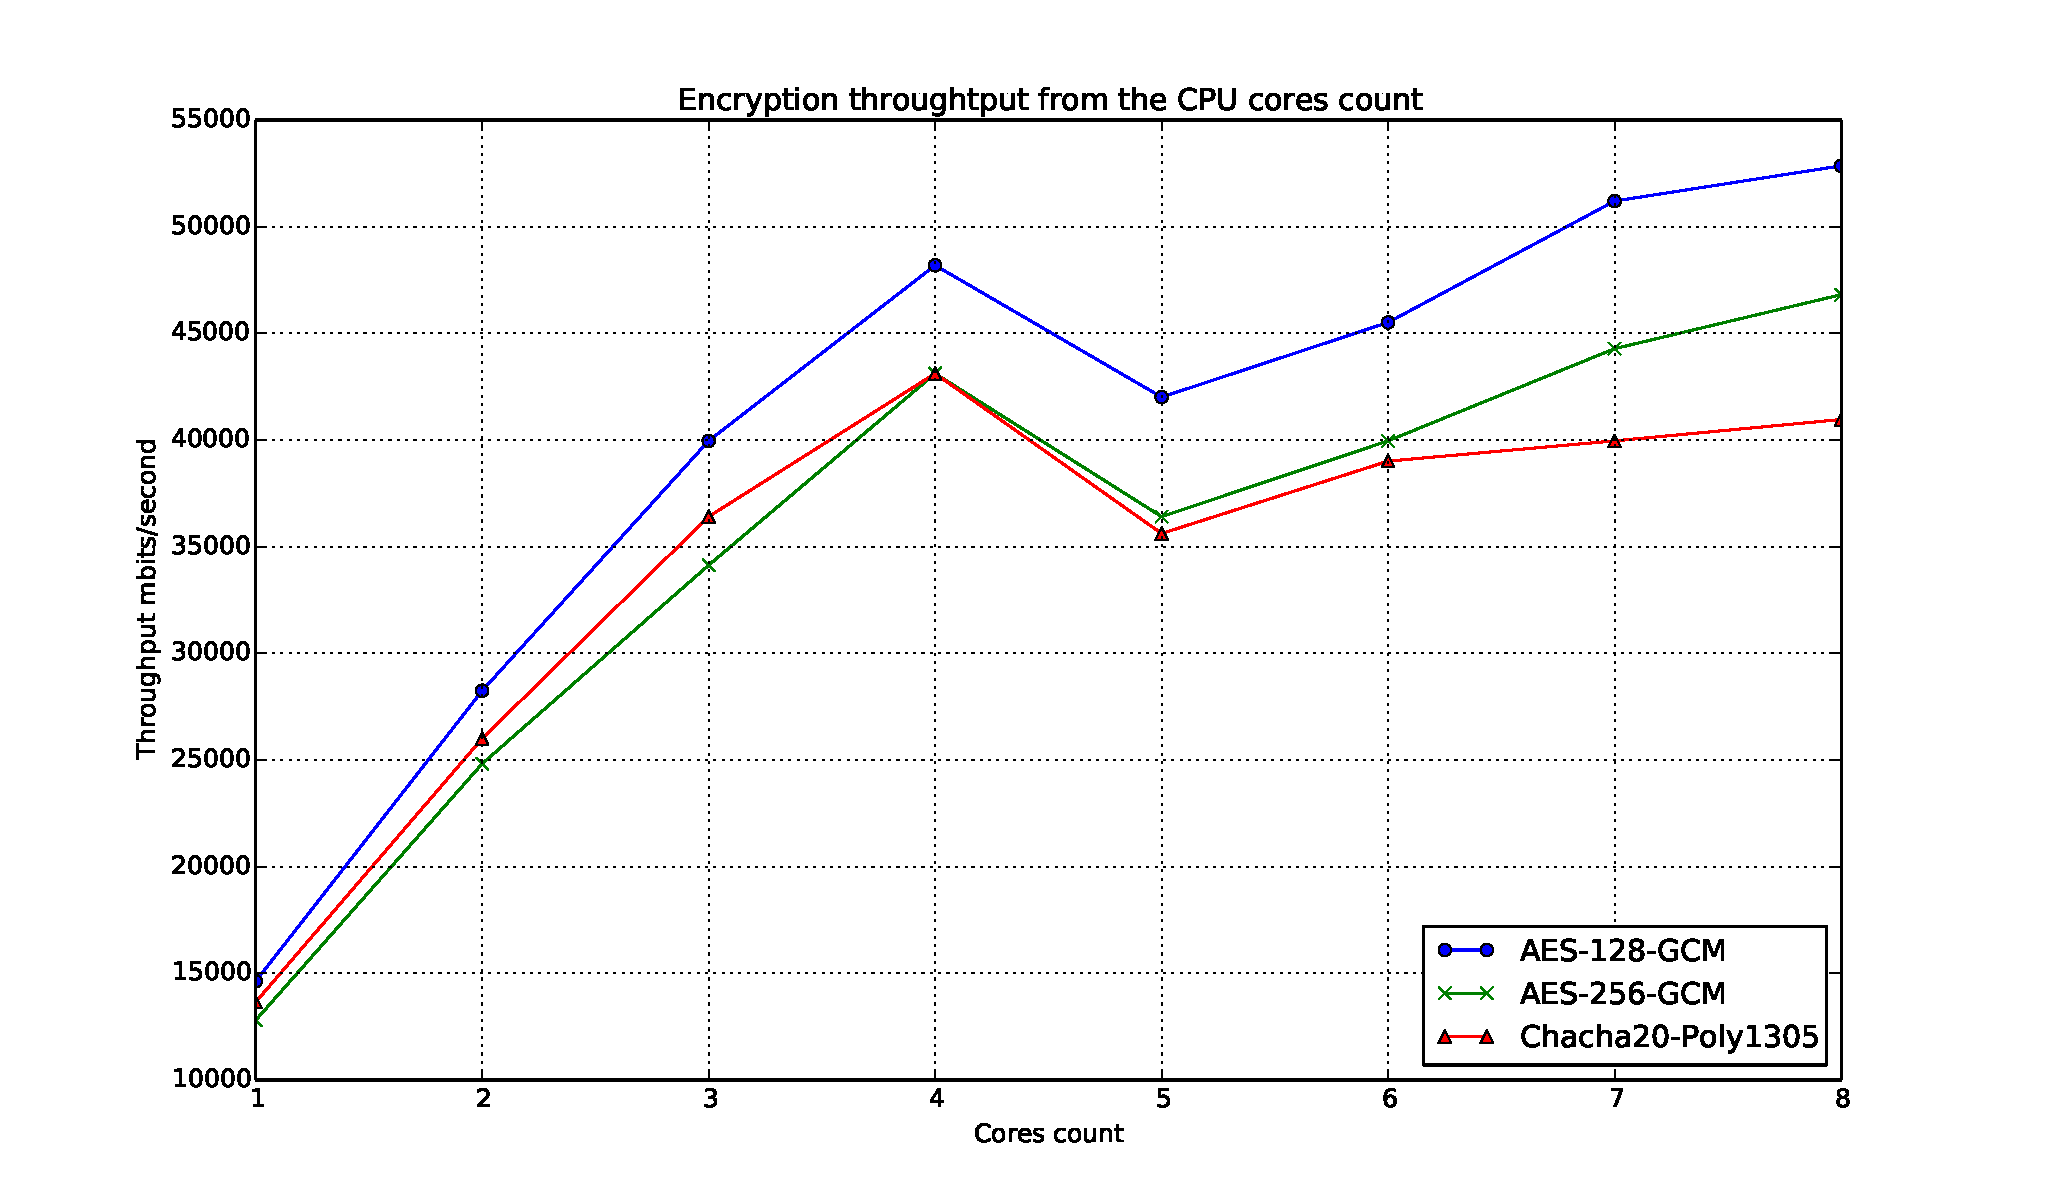
\includegraphics[height=0.6\textheight]{perf-i7.pdf}
\caption{Core-i7 4770, 3.5 GHz, 8 CPU cores}
\end{figure}
\end{frame}

\begin{frame}
\frametitle{How expensive is encryption nowadays}
\framesubtitle{Hardware performance}
Pre-historic ages: Core2 quad (SSE3):
\begin{figure}[H]
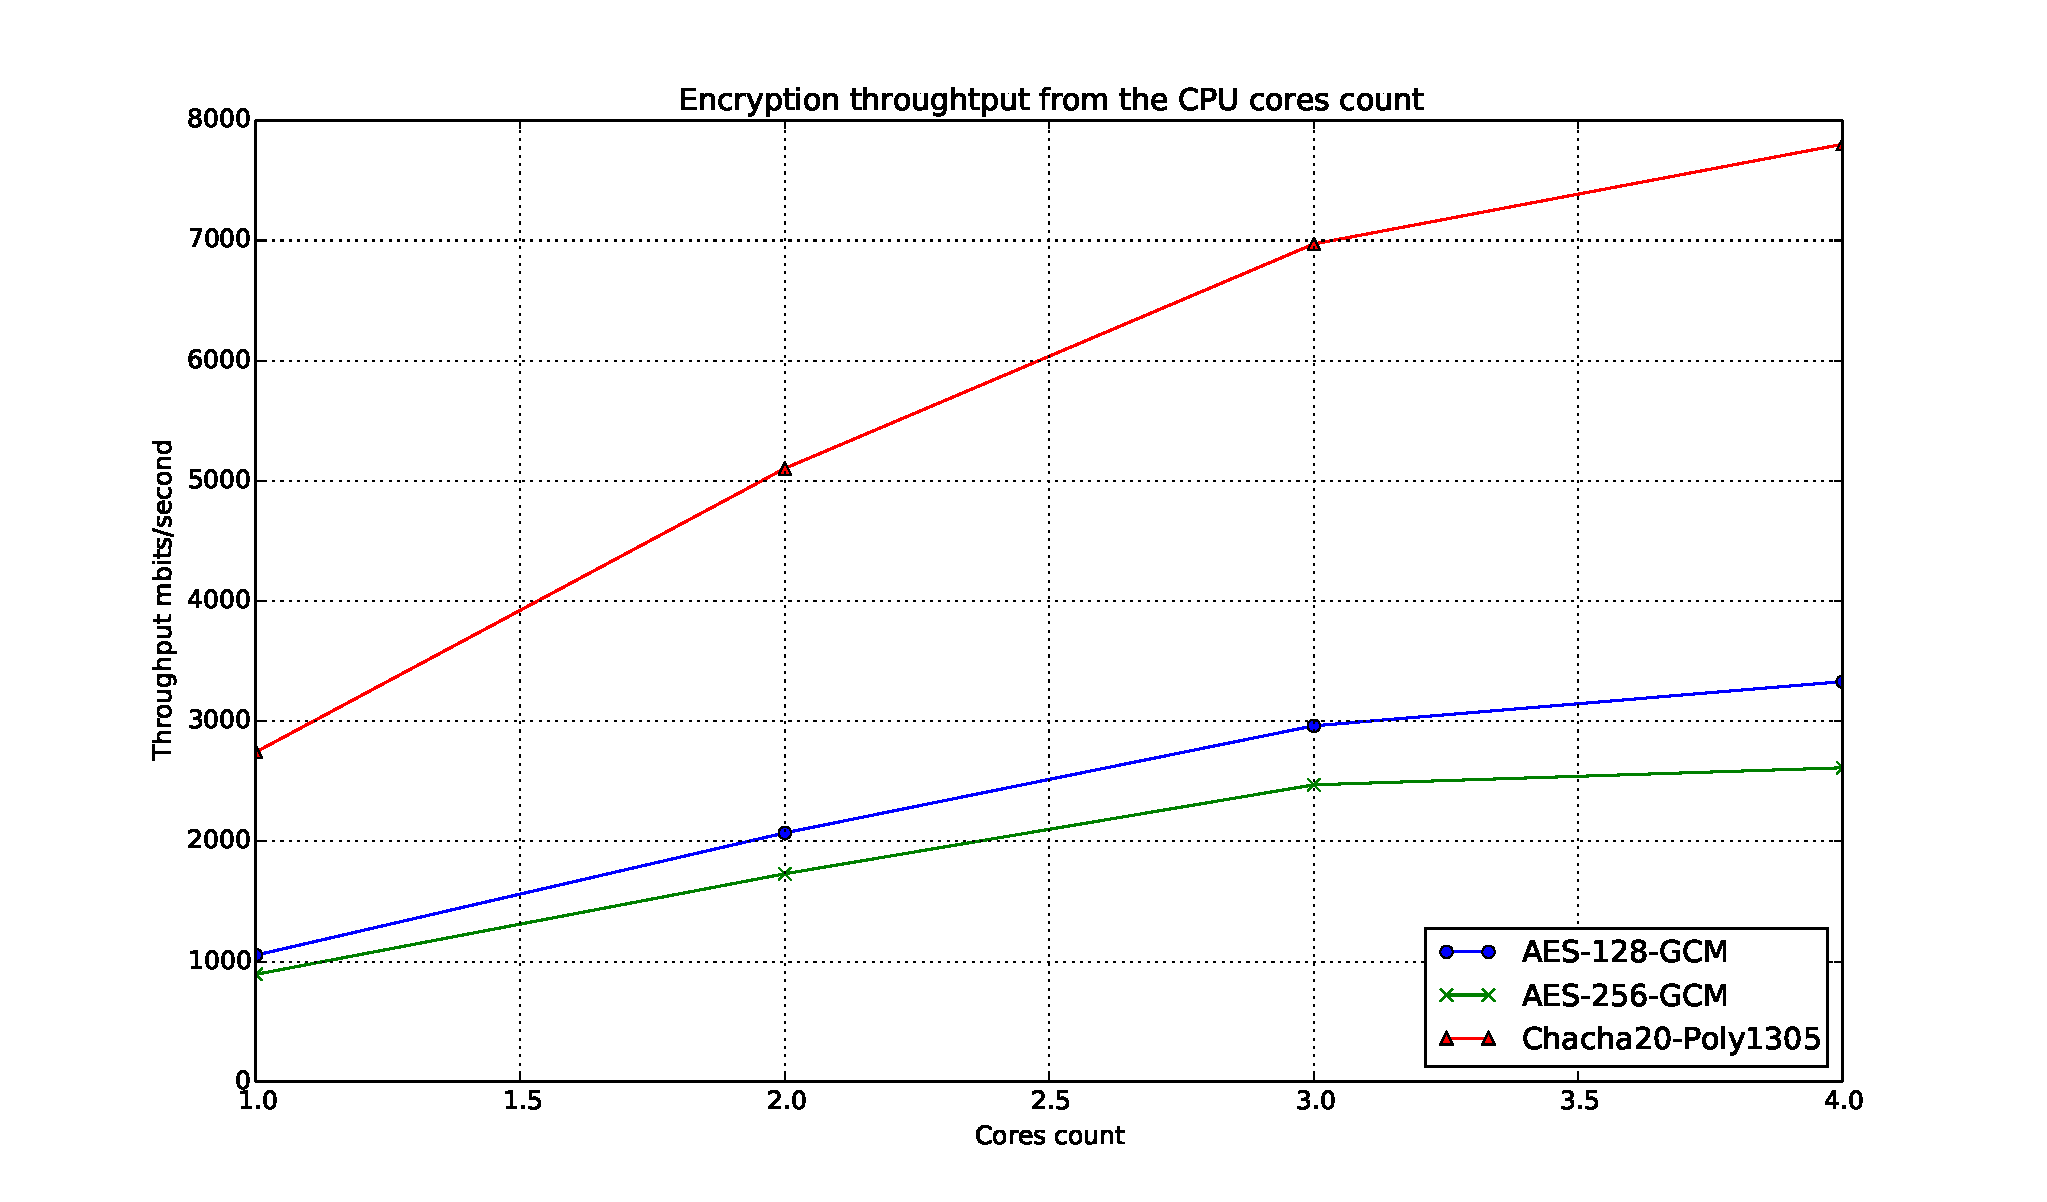
\includegraphics[height=0.6\textheight]{perf-c2.pdf}
\caption{Core2-quad, 1.5 GHz, 4 CPU cores}
\end{figure}
\end{frame}

\begin{frame}
\frametitle{How expensive is encryption nowadays}
\framesubtitle{Algorithm performance} 
\cipher{3DES}:
	\begin{itemize}
	\item very small block size (64 bits)
	\item need to rekey after 32 GB data
	\item need some additional MAC algorithm
	\item terribly slow
	\end{itemize}
\end{frame}

\begin{frame}
\frametitle{How expensive is encryption nowadays}
\framesubtitle{Algorithm performance} 
\cipher{ChaCha20}:
\begin{figure}[H]
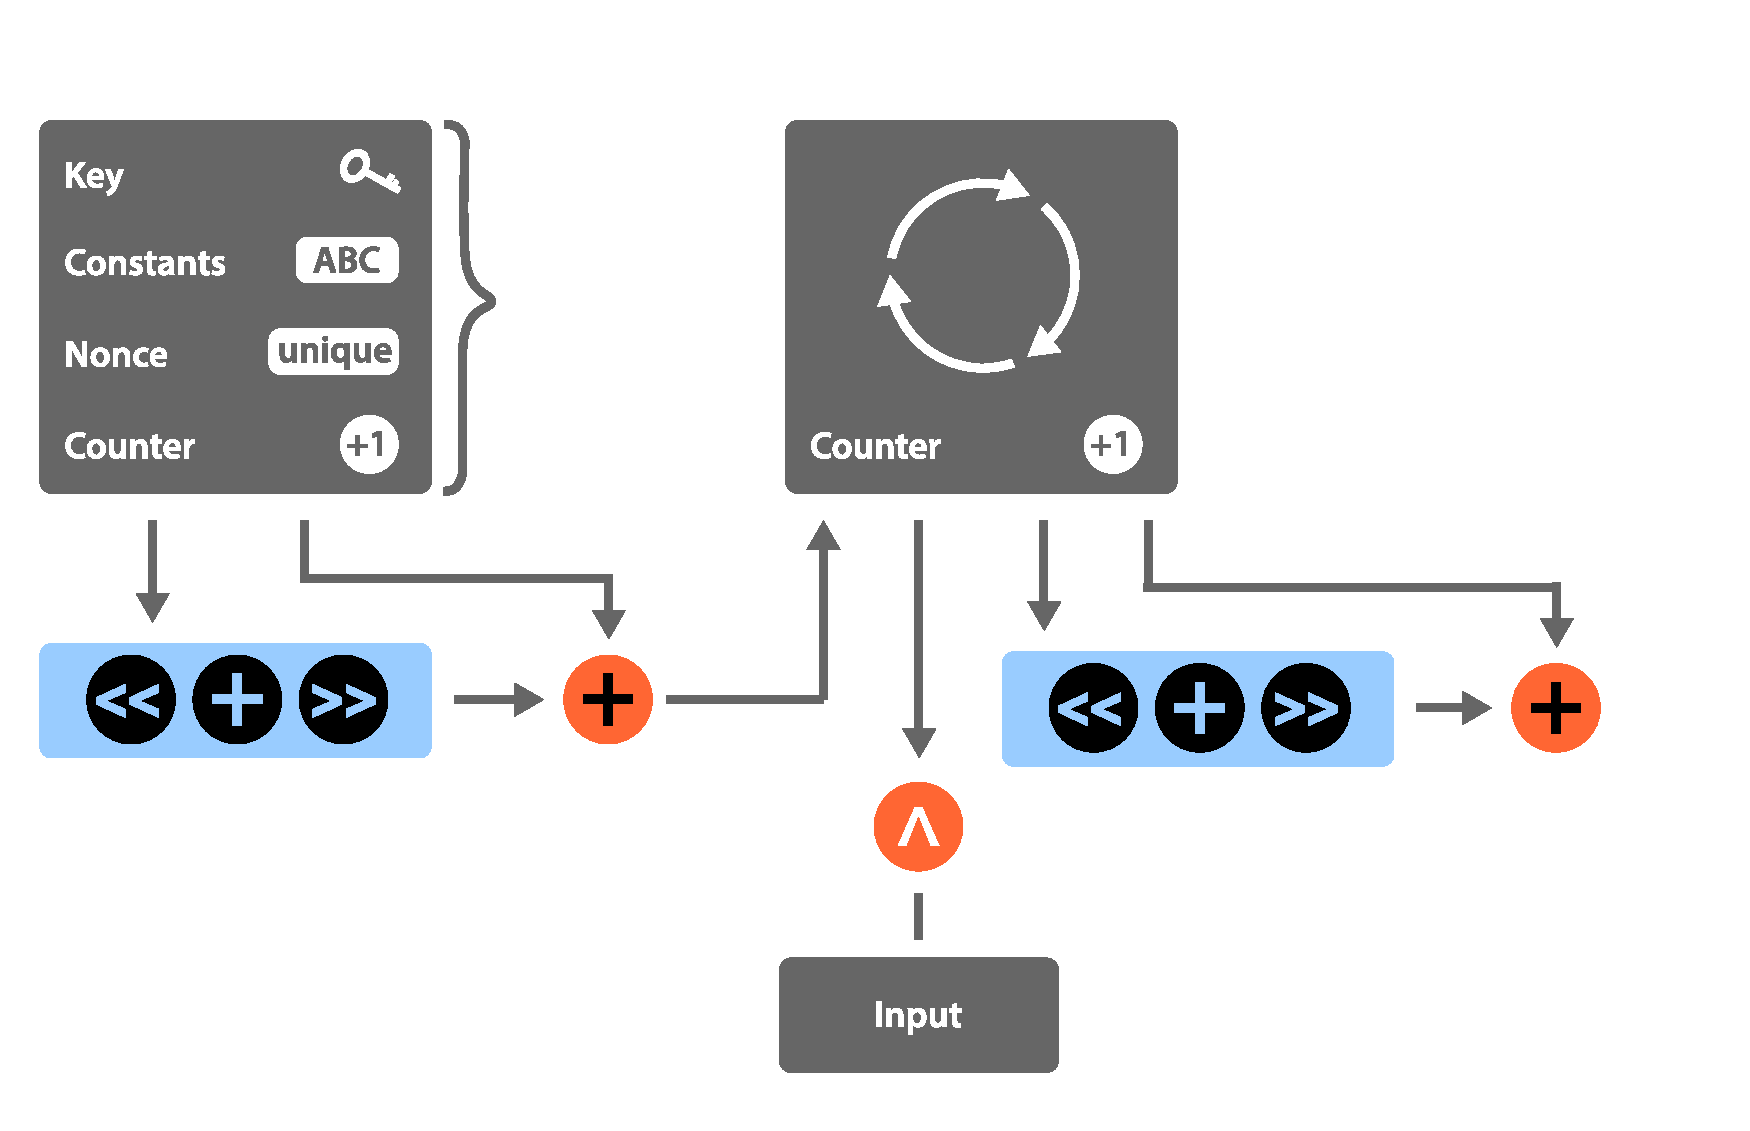
\includegraphics[height=0.7\textheight]{chacha.pdf}
\end{figure}
\end{frame}

\begin{frame}[fragile]
\frametitle{How expensive is encryption nowadays}
\framesubtitle{Algorithm performance} 
\cipher{ChaCha20} round:
\begin{tiny}
\begin{minted}{c}
void qr(a,b,c,d) {
    a += b; d ^= a; d <<<= 16;
    c += d; b ^= c; b <<<= 12;
    a += b; d ^= a; d <<<= 8;
    c += d; b ^= c; b <<<= 7;
}

for (i = chacha_rounds;i > 0;i -= 2) {
    qr(x0, x4, x8,x12)
    qr(x1, x5, x9,x13)
    qr(x2, x6,x10,x14)
    qr(x3, x7,x11,x15)
    qr(x0, x5,x10,x15)
    qr(x1, x6,x11,x12)
    qr(x2, x7, x8,x13)
    qr(x3, x4, x9,x14)
}
\end{minted}
\end{tiny}
\begin{itemize}
\item<2-> Each round modifies the whole block
\item<2-> Each quarter round operation is independent from others in the round
\item<2-> Efficient diagonal optimizations for SSE/AVX/AVX512
\item<2-> Need even number of rounds (20 or 12 typically)
\end{itemize}
\end{frame}

\begin{frame}
\frametitle{How expensive is encryption nowadays}
\framesubtitle{Algorithm performance} 
Advantages of \cipher{ChaCha20}:
\begin{itemize}
\item clear and simple design
\item 512 bits of block size (up to $2^{70}$ bytes before rekeying)
\item fit very well for vectorized operations (and especially for AVX)
\end{itemize}
Current usage of \cipher{ChaCha20-Poly1305}:
\begin{itemize}
\item openssh
\item libressl and boringssl
\item libottery fast pseudo-random generator
\item OpenBSD \funcname{arc4random}
\item Chrome browser
\item proposed IETF standard for TLS and IPSEC
\end{itemize}
\end{frame}

\begin{frame}[fragile]
\frametitle{How expensive is encryption nowadays}
Protocols performance:
\begin{figure}[H]
\centering
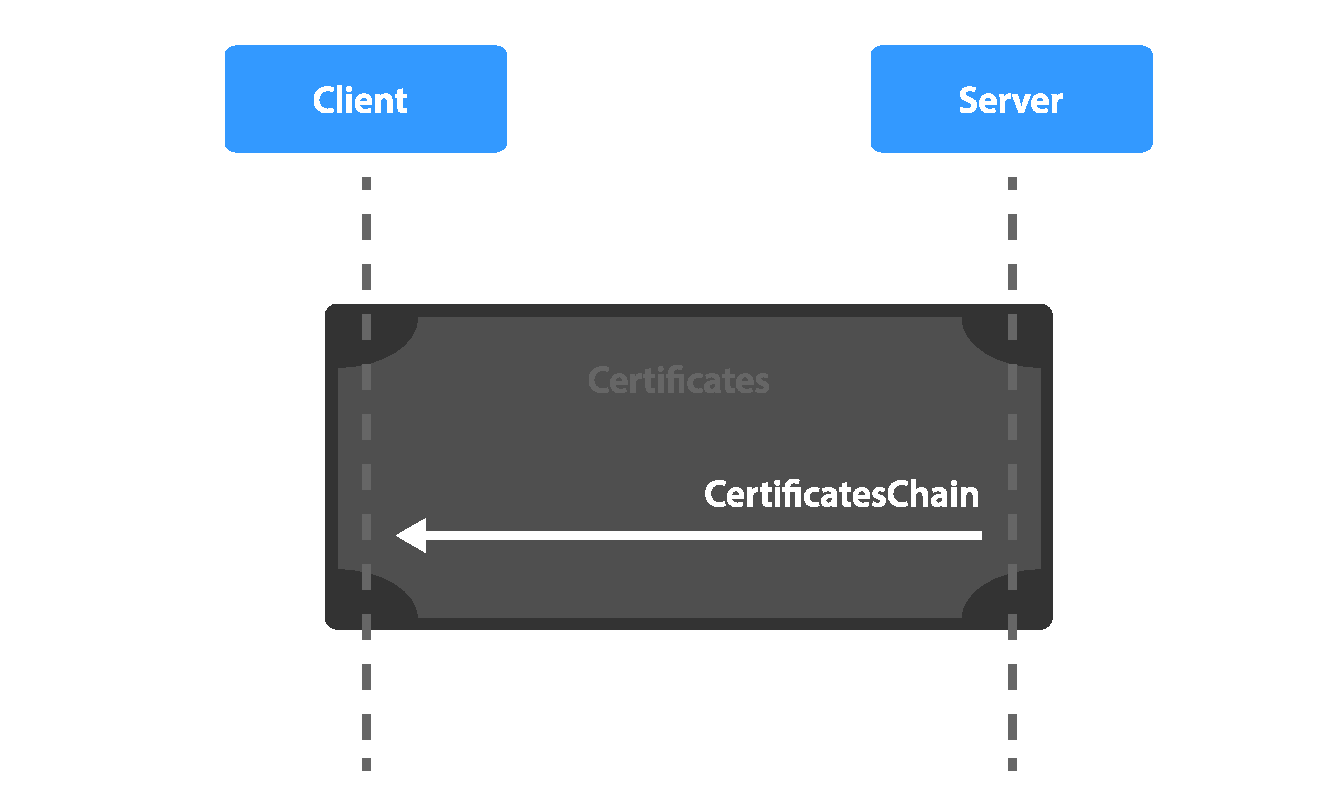
\includegraphics[height=0.6\textheight]{tls.pdf}
\caption{TLS connection establishment}
\end{figure}
\end{frame}

\begin{frame}
\frametitle{Performance: current progress}
\begin{itemize}
\item<1-> Experimental support of \cipher{AES-GCM} in OpenBSD and FreeBSD (by John-Mark 
Gurney), problems with additional registers saving on context switch
\item<2-> Support of \cipher{ChaCha20-Poly1305} in libressl, boringssl and libgrypt (and 
gnutls)
\item<3-> Deprecating of \cipher{RC4} in OpenBSD (proposed in FreeBSD and NetBSD as well)
\end{itemize}
\end{frame}

\begin{frame}
\frametitle{Building secure systems}
General problems when building secure systems:
\begin{itemize}
\item<1-> Curse of backward compatibility
\item<2-> Complex and inconsistent API (OpenSSL)
\item<3-> Bad default settings
\item<3-> Permit everything by default
\end{itemize}
\end{frame}

\begin{frame}
\frametitle{Building secure systems}
\framesubtitle{Backward compatibility}
\begin{itemize}
\item<1-> Protocols design flaws
\item<2-> Poor algorithmic choices:
	\begin{itemize}
	\item Reduce security
	\item Remove important properties, e.g. forward secrecy property
	\item Can be very slow (\cipher{3DES}) and hence lead to computational DoS
	\end{itemize}
\end{itemize}
\end{frame}

\begin{frame}
\frametitle{Building secure systems}
\framesubtitle{Backward compatibility}
Practical example - LibreSSL replacement of OpenSSL
\begin{itemize}
\item Legacy API - \cipher{DES} support in OpenLDAP
\item Invalid random number generators - \funcname{RAND\_egd} which is valid merely for Linux (Python, Curl, Wget and many other ports)
\item SSL3 and even SSL2 support (Curl)
\item Unnecessary engine functions (many ports, including apache) 
\end{itemize}

Practically \textit{all} the issues listed are also valid for the upcoming OpenSSL 1.0.2 
branch.
\end{frame}

\begin{frame}
\frametitle{Building secure systems}
\framesubtitle{Design flaws example: TLS}
Encrypt and MAC choice.
%XXX demonstrate
\begin{itemize}
\item Sensitive to side attacks (PaddingOracle, LuckyThirteen)
\item Inefficient computation
\item No integrity on ciphertext (can be dangerous if used with malleable ciphers)
\item No protection against the attacks to a cipher itself
\end{itemize}
Proposed: encrypt-then-mac extension in RFC7366.
\end{frame}

\begin{frame}[fragile]
\frametitle{Building secure systems}
\framesubtitle{CBC mode}
\begin{figure}[H]
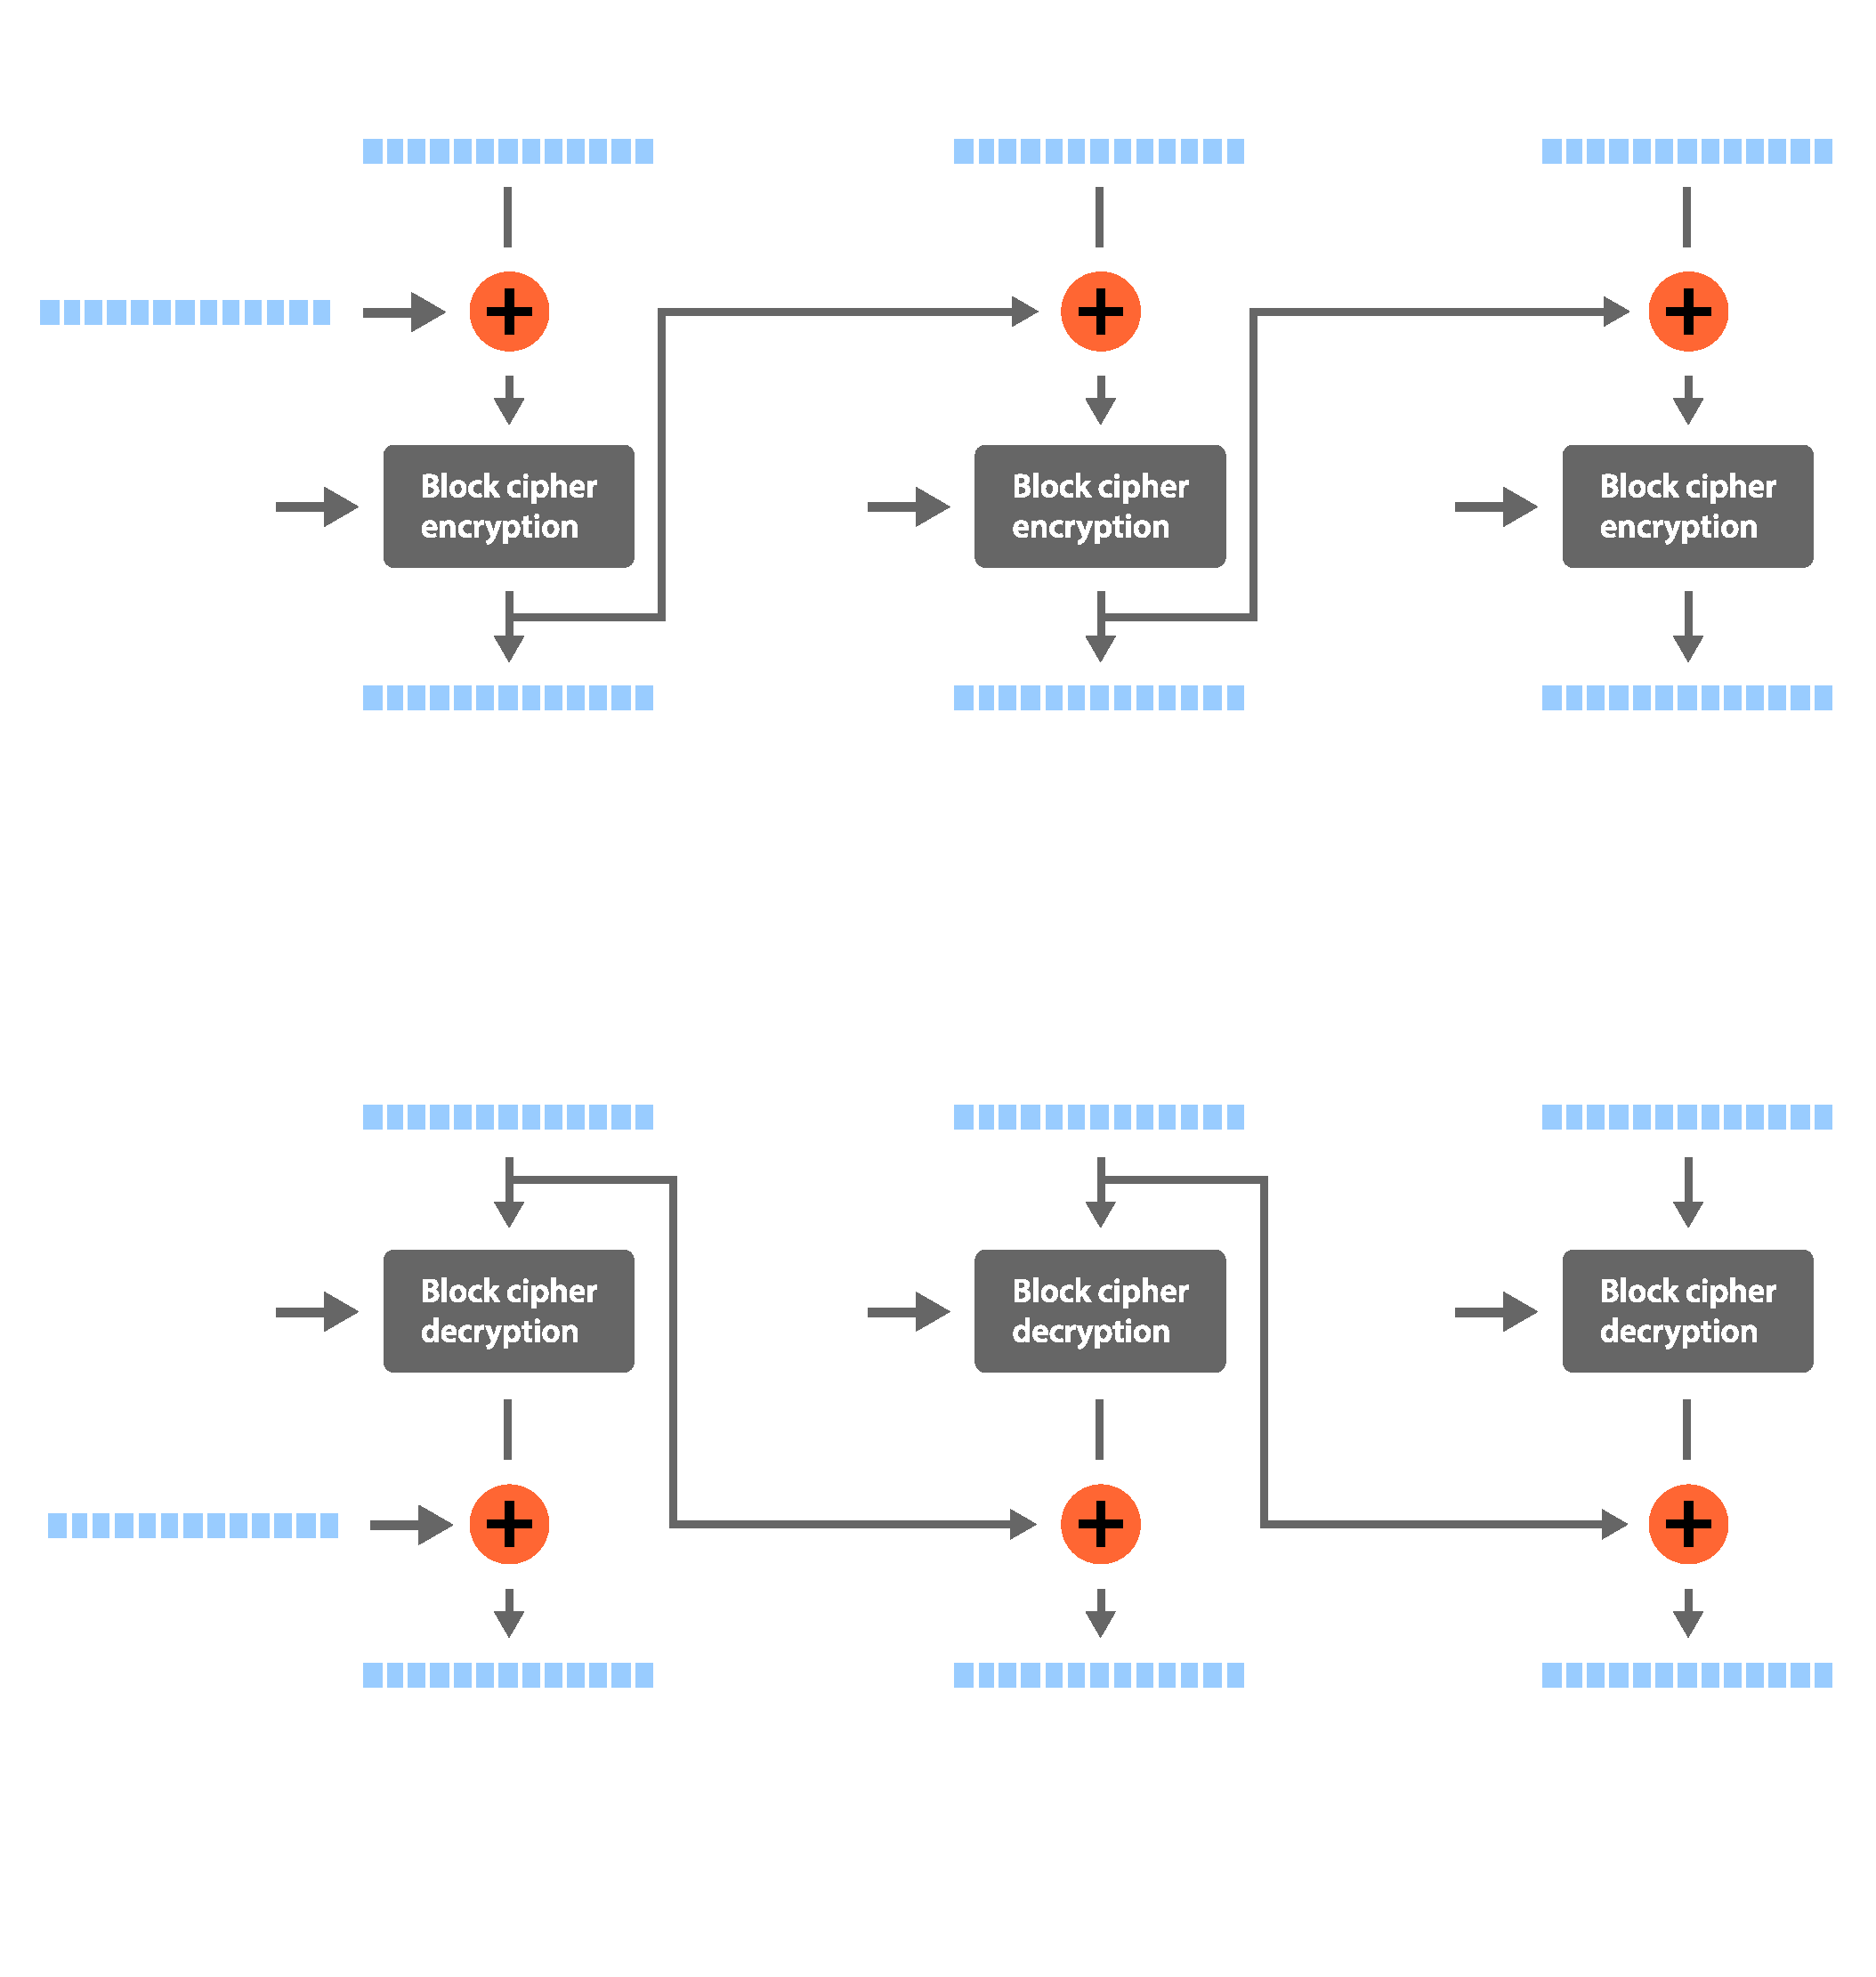
\includegraphics[height=0.85\textheight]{cbc.pdf}
\end{figure}
\end{frame}

\begin{frame}
\frametitle{Building secure systems}
\framesubtitle{CBC mode}
\begin{itemize}
\item Assumes that cipher is secure for all data even if it is controlled by an attacker
\item Decryption differs from encryption
\item Cannot be computed in parallel
\item Needs careful padding (Poodle attack)
\end{itemize}
Proposed: use ciphers in counter mode only (not compatible with old browsers)
\end{frame}

\begin{frame}[fragile]
\frametitle{Building secure systems}
\framesubtitle{Counter mode}
\begin{figure}[H]
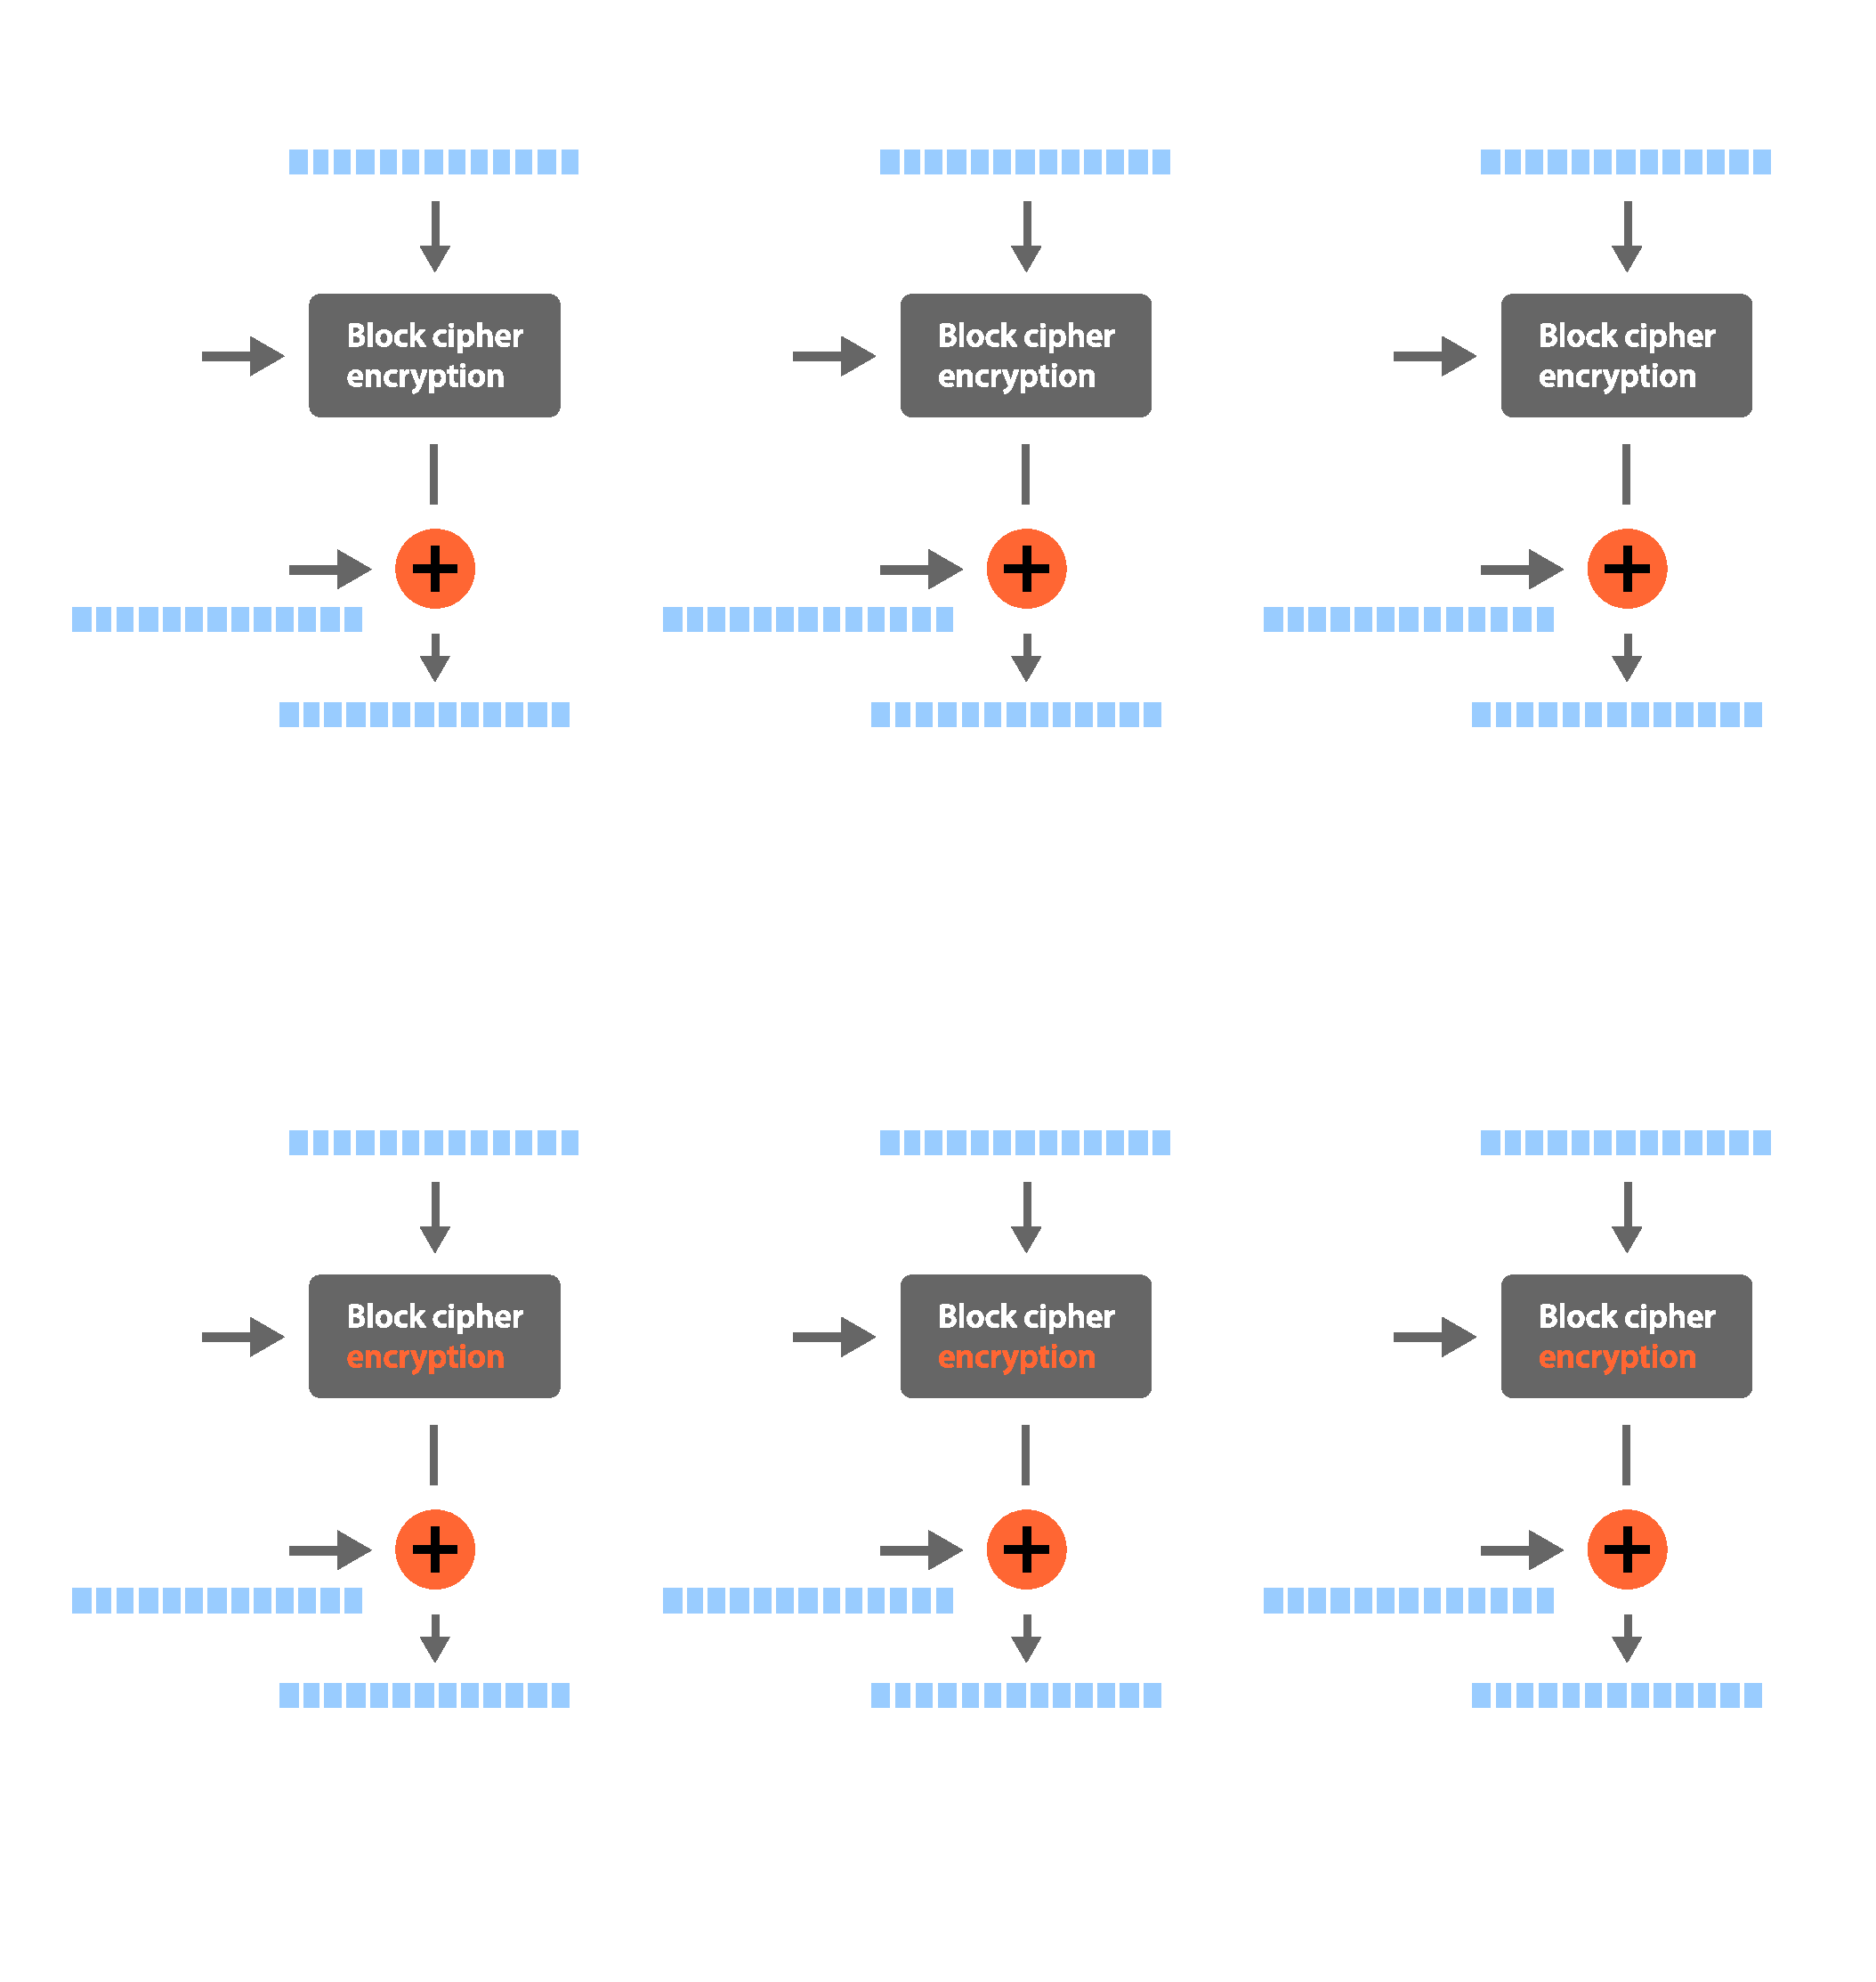
\includegraphics[height=0.85\textheight]{ctr.pdf}
\end{figure}
\end{frame}

\begin{frame}
\frametitle{Building secure systems}
\framesubtitle{Counter mode}
\begin{itemize}
\item Ciphers accepts only deterministic counter input
\item Decryption is equal to encryption
\item Can be computed in parallel
\item Need to ensure that the counter never ever repeats
\end{itemize}
\end{frame}

\begin{frame}
\frametitle{Building secure systems}
\framesubtitle{API design flaws}
\begin{itemize}
\item<1-> all software contain mistakes
\item<2-> complicated API increases chance of mistakes some of them are security 
vulnerabilities
\item<3-> inconsistent API provokes misusage
\item<4-> always prefer simple and widely used libraries (meaning \textbf{do not 
implement your own cryptographic library})
\end{itemize}
\end{frame}

\begin{frame}[fragile]
\frametitle{Building secure systems}
\framesubtitle{API design flaws: OpenSSL}
Certificates verification.
\begin{itemize}
\item Terribly complicated - just look at the documentation of 
\funcname{SSL\_set\_verify} and auxiliary function \funcname{SSL\_set\_ex\_data}:
\begin{tiny}
\begin{minted}{c}
ssl = X509_STORE_CTX_get_ex_data(ctx, SSL_get_ex_data_X509_STORE_CTX_idx());
mydata = SSL_get_ex_data(ssl, mydata_index);
\end{minted}
\end{tiny}
\item You need to check certificate CN manually (not even covered in the example in 
the manual page)
\item You need manually check all extensions such as SNI or ALPN (and many openssl users 
fail to do it correctly)
\end{itemize}
\end{frame}

\begin{frame}[fragile]
\frametitle{Building secure systems}
\framesubtitle{API design flaws: OpenSSL}
Macro based API.
\begin{itemize}
\item Inconsistent: 
\begin{enumerate}
\item Many ways to do the same thing, for example \textbf{EVP} and legacy and obsoleted 
interfaces: \funcname{EVP\_PKEY\_encrypt} and \funcname{RSA\_public\_encrypt}.
\item Confusing names \funcname{PEM\_read\_RSAPublicKey}, 
\funcname{PEM\_read\_RSA\_PUBKEY} 
and \funcname{PEM\_read\_PUBKEY}
\end{enumerate}
\item Dangerous pointers API:
\begin{tiny}
\begin{minted}{c}
unsigned char *sk, *p;
size_t sklen;

sklen = i2d_ECPrivateKey(ec_key, NULL);
sk = malloc(sklen);
p = sk;
i2d_ECPrivateKey(ec_key, &p);
/* p is now at the end of sk */
\end{minted}
\end{tiny}
\end{itemize}
\end{frame}

\begin{frame}[fragile]
\frametitle{Building secure systems}
\framesubtitle{API design flaws: some practical advices}
Higher level libraries:
\begin{itemize}
\item libtls from OpenBSD (formely ressl):
\begin{tiny}
\begin{minted}{c}
#include <tls.h>

struct tls *tls_client(void);
int tls_connect(struct tls *ctx, const char *host, const char *port);
int tls_read(struct tls *ctx, void *buf, size_t buflen, size_t *outlen);
int tls_write(struct tls *ctx, const void *buf, size_t buflen, size_t *outlen);
int tls_close(struct tls *ctx);
\end{minted}
\end{tiny}
\item libsodium (for generic encryption/signing)
\begin{tiny}
\begin{minted}{c}
/* Encrypt */
memset(out, '\0', crypto_box_ZEROBYTES);
memcpy(out + crypto_box_ZEROBYTES, plain, length);
rc = crypto_box(enc, out, crypto_box_ZEROBYTES + length, nonce, pk, sk);

/* Decrypt */
memset(in, '\0', crypto_box_BOXZEROBYTES);
memcpy(in + crypto_box_BOXZEROBYTES, enc, length);
rc = crypto_box_open(plain, in, crypto_box_BOXZEROBYTES + length, nonce, pk, sk);
if (rc != 0) /* Verification error */
\end{minted}
\end{tiny}
\end{itemize}
\end{frame}

%\begin{frame}[fragile]
%\frametitle{Building secure systems}
%\framesubtitle{API design flaws: additional materials}
%\begin{enumerate}
%\item `The most dangerous code in the world: validating SSL certificates in non-browser 
%software' by Georgiev, Boneh, Shmatikov et al.
%\item `Lucky Thirteen: Breaking the TLS and DTLS Record Protocols': 
%\end{enumerate}
%\end{frame}

\begin{frame}
\frametitle{Building secure systems}
\framesubtitle{Insecure default settings}
\begin{itemize}
\item Enable all possible extensions even if they are not used (Heartbleed)
\item Be compatible with old and broken systems, notably Windows XP (SSL Poodle)
\item Prefer client settings
\item Too many sources of trust
\end{itemize}
\end{frame}

\begin{frame}[fragile]
\frametitle{Building secure systems}
\framesubtitle{Secure defaults: basics}
\begin{itemize}
\item Explicitly set order and disable weak ciphersuites:
	\begin{itemize}
	\item Disable SSLv3 if possible (or enable \funcname{TLS\_FALLBACK\_SCSV} in both 
	client and server)
	\item Always prefer key exchange with ephemeral keys
	\item Disable 3DES to avoid computational DoS
	\item Prefer strong cipher suites, e.g. 
	{\scriptsize 
	\texttt{\cipher{EECDH+ECDSA+CHACHA20-POLY1305:EECDH+ECDSA+AESGCM}}
	}
	\end{itemize}
\item Set sane expiration for keys
\item Use elliptic curve cryptography (if possible)
\item Be very careful when choosing entropy source: e.g. prefer \funcname{getentropy(2)} 
call in OpenBSD to \texttt{/dev/random} especially with sandboxing or containers
\end{itemize}
\end{frame}

\begin{frame}[fragile]
\frametitle{Building secure systems}
\framesubtitle{Advanced topics}
Some additional modern technologies to build secure systems.
\begin{itemize}
\item DANE/DNSSEC allows to move from CA and PKI trust relationships to DNS trust
\begin{itemize}
\item DNSSEC requires recursion being used for all DNS clients
\item Has some risk of replay based attacks (especially in clouds)
\item Increases the risk of DNS amplification attacks (can be mitigated by rate-limits)
\item Implies ECC if you want to store the whole certificate in DNS (for speed)
\item Requires additional DNS requests
\item Can be filtered by middleboxes
\item Still fragile if your 1-st level zone provider is not trusted
\end{itemize}
\item Use opportunistic transport layer encryption: tcpcrypt
\item Use type safe TLS libraries: ocaml-tls, mitls
\end{itemize}
\end{frame}

\begin{frame}[fragile]
\frametitle{Building secure systems}
\framesubtitle{Advanced topics: DNS security}
DNSCurve: complete DNS traffic encryption
\begin{itemize}
\item Encrypts and authorize all traffic between client and authoritative server
\item Breaks all intermediate caches if enabled
\item Requires global deployment
\end{itemize}
DNSCrypt: encrypt the last mile of DNS exchange
\begin{itemize}
\item Encrypts and protects all communications between client and recursor
\item Can be used with DNSSEC
\item Can be used even without explicit authorization but still protects from passive 
snooping (e.g. in open wireless networks)
\end{itemize}
\end{frame}

\begin{frame}[fragile]
\frametitle{Building secure systems}
\framesubtitle{Advanced topics: Transport encryption}
tcpcrypt - transport layer encryption (MAC is added for each packet as TCP option)
\begin{itemize}
\item Opportunistically encrypts all TCP connection invisible for applications
\item Compatible\footnote{almost} with middleboxes in the Internet
\item Requires zero setup and establish encrypted connections automatically
\item Faster than SSL
\end{itemize}
Disadvantages:
\begin{itemize}
\item No authority checks (can be done via DANE however)
\item Not supported by the most of TCP stacks (experimental linux kernel support and 
divert socket concept version)
\item Increases TCP handshake duration to 4 RTT
\item Incompatible with TSO
\end{itemize}
\end{frame}

\begin{frame}
\vfill\vfill\centering
\emph{Questions?} \\[4pt]
\url{vsevolod@FreeBSD.org}
\vfill\vfill
\end{frame}

\end{document}